% xelatex
\documentclass[12pt]{article}
\usepackage[bf,center]{titlesec}
\usepackage[utf8]{inputenc}
\usepackage{enumitem}
\usepackage{fancyhdr}
\usepackage{gensymb} % grādu simbols
\usepackage{geometry}
\usepackage{graphicx}
\usepackage{hyperref}
\usepackage{indentfirst}
\usepackage{multicol}
\usepackage{ragged2e}
\usepackage{secdot}
\usepackage{tabularx}
\usepackage{tcolorbox}
\usepackage{tocloft}


\hypersetup{
	colorlinks=true,
	linkcolor=black,
	urlcolor=blue
}

\urlstyle{rm}

\titlespacing*{\section}{0pt}{0pt}{1.5pt}
\titlespacing*{\subsection}{0pt}{0.5\baselineskip}{1.5pt}
\titlespacing*{\subsubsection}{0pt}{0.5\baselineskip}{1.5pt}
\titleformat{\section}{\large \bfseries \centering}{\thesection.}{1em}{} % section formatting
\titleformat{\subsection}{\normalsize \bfseries
	\centering}{\thesubsection.}{1em}{} % subsection formatting
\titleformat{\subsubsection}{\normalsize \bfseries
	\centering}{\thesubsubsection.}{1em}{} % subsubsection formatting
\geometry{a4paper, left=3cm, right=2cm, top=3cm, bottom=2cm}
\pagestyle{fancy}
\fancyhead{}
\fancyfoot{}
\fancyfoot[C]{\thepage}
\renewcommand{\headrulewidth}{0pt}
\linespread{1.3}
\setlength{\parindent}{1cm}
\setlength{\parskip}{0pt}
\renewcommand{\contentsname}{\hspace*{\fill}\bfseries\large Table of contents\hspace*{\fill}} 
\renewcommand{\cfttoctitlefont}{\centering\bfseries\large} % Remove \bfseries from ToC title
\renewcommand{\cftsecfont}{} % Remove \bfseries from section titles in ToC
\renewcommand{\cftsecpagefont}{} % Remove \bfseries from section titles' page in ToC
\renewcommand{\cftsecleader}{\cftdotfill{\cftsecdotsep}}
\renewcommand\cftsecdotsep{\cftdot}
\renewcommand\cftsubsecdotsep{\cftdot}
\renewcommand{\cftsecaftersnum}{.} % dot after section number
\renewcommand{\cftsubsecaftersnum}{.}

\begin{document}
    \begin{titlepage}
    \thispagestyle{empty}
    \begin{center}
        \vspace*{2cm}
        \begin{large}\textbf{UNIVERSITY OF LATVIA}

            \textbf{FACULTY OF COMPUTING}

            \vfill
            \textbf{Open-Source Software Database (OSSDB)}
        \end{large}

        \vfill
        \textbf{Databases and Information Systems Fundamentals}
    \end{center}
    \vspace{4cm}
    \begin{flushright}
        Author: \textbf{Kristiāns Francis Cagulis}

        Student ID No.: kc22015

    \end{flushright}
    \vspace{1cm}
    \begin{center}
        RIGA 2023
    \end{center}
\end{titlepage}


    \pagebreak
	\tableofcontents
    \thispagestyle{empty}
    % \input{./TeX-files/before-content/abstract.tex}
    \setcounter{page}{2}
    \pagebreak
\section{Introduction}
Open-source software has grown in popularity over the years due to its collaboration, innovation, and cost savings benefits.
Typically, open-source software is created and maintained by a community of developers who work together to improve their projects, share experiences and contribute to their growth.
As a result, there are now dozens of open source projects covering everything from software development to data science, robotics and more.

However, it can be difficult to keep track of all the open source projects available.
Project leaders and maintainers often struggle to find contributors to help build projects, while contributors struggle to find projects that match their interests and expertise.
This is where the Open-Source Software Database (OSSDB) comes into play.

The OSSDB is a comprehensive online platform that acts as a central repository for tracking and managing open source projects.
This database provides project listings, search capabilities, filters, user profiles, etc. to help contributors find projects to contribute to
and for project leaders and maintainers to find contributors to help build the project.
The OSSDB aims to provide a platform that fosters collaboration, transparency and innovation in the open-source software community.

The OSSDB itself will be an open source project, and as such will be free and accessible to everyone.
This approach is in line with the open source philosophy, which encourages collaboration, transparency and community-driven innovation.
This project aims to encourage more people to get involved in open source projects and contribute to the growth of the community.
The project will rely on contributions and feedback from the community to continuously improve and refine the OSSDB.

    \pagebreak
\section{Features}
The platform will offer project listings that include project description, contributor,
license types, code hosting platforms, operating systems on which the app can run,
programming languages, stars, and project tags.
Users will be able to easily locate projects using the search and filter functionality that will allow them
to search by name, keyword, programming language, project tag, license type, and contributor.

The FOSSDB intends to implement several features in the long term to improve the platform's
functionality and user experience.
These features include notifications, a review and rating system and a dedicated website. 

Users will be able to receive notifications when other users are looking to collaborate
on a project to which they are interested in or have contributed to.
This will allow users to connect with other developers who share their interests,
fostering collaboration and innovation in the open-source software community. 

The rating and reviewing feature will allow users to give feedback and rate the
projects they have used or contributed to.
This will help other users make informed decisions about which projects
to use and contribute to, based on the experiences of other users. 

Finally, there are plans to create a dedicated website for the platform,
which will act as a central hub for discovering open-source software projects. 
 % Features
    \pagebreak
\section{Requirements}

\begin{itemize}
    \item User Authentication: FOSSDB must provide user authentication to allow users to
    create and manage their profiles.

    \item Project creation: Registered users should be able to create projects and provide
    basic information about the project, such as project name, description, licenses,
    programming languages used, hosting platform, and operating systems supported.

    \item Star Rating: The FOSSDB must allow users to rate projects by assigning them stars.
    The rating system should be able to prevent multiple ratings from the same user.

    \item Tagging: FOSSDB should allow users to tag projects with relevant keywords
    to assist in searching and filtering.

    \item Licensing: FOSSDB should maintain a database of open source licenses and
    their associated details, including short name, full name, URL, and description.
    All projects listed in FOSSDB must be licensed under a FOSS license.
    Examples of FOSS licenses include the MIT License, the GNU General Public License (GPL),
    and the Apache License.

    \item Programming Languages: The FOSSDB should maintain a database of programming
    languages and their usage amount for each project.

    \item Hosting Platforms: The FOSSDB should maintain a database of hosting platforms
    and each project hosting platform associated URL.

    \item Operating Systems: The FOSSDB should maintain a database of operating systems and
    their associated details, including name, description, version.
\end{itemize}
 % Requirements
    \pagebreak
\section{Conceptual model}

\begin{figure}[h]
  \centering
  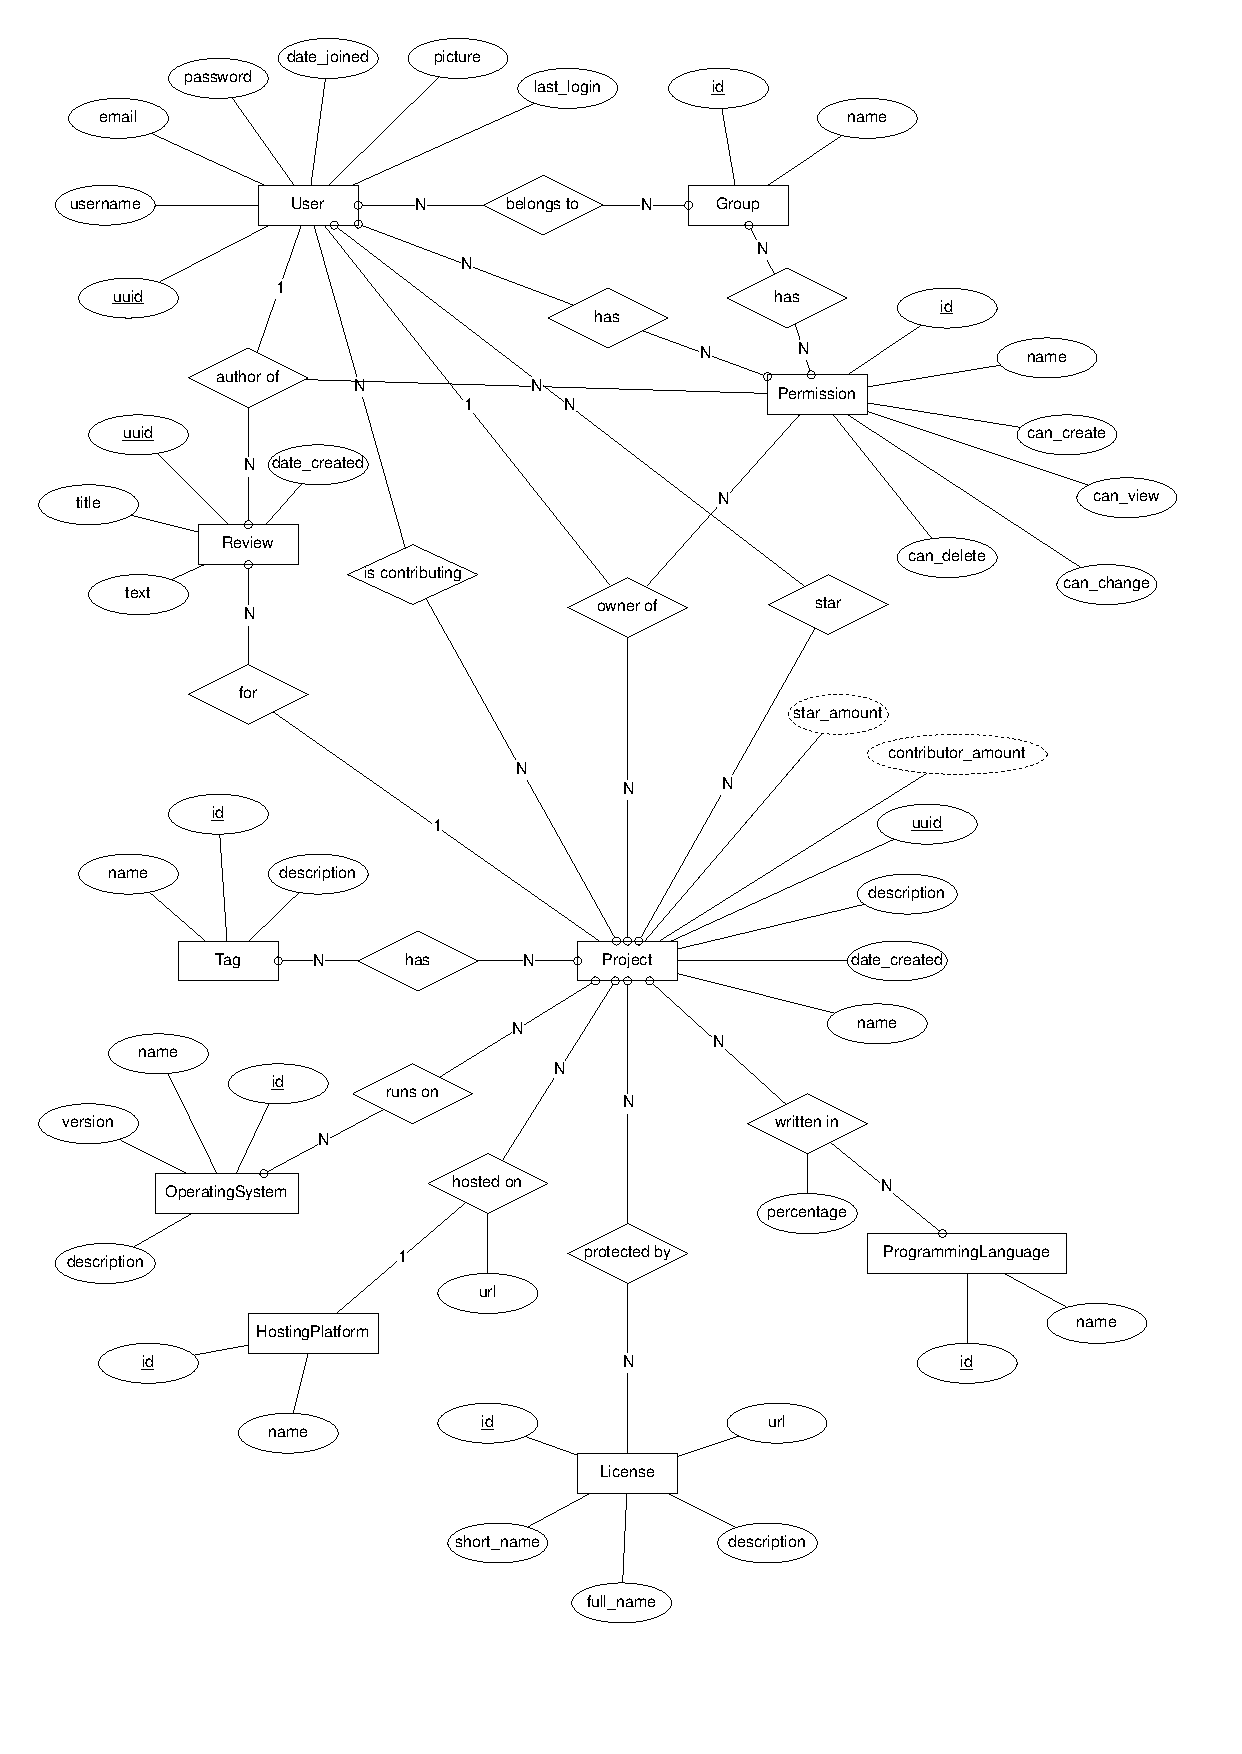
\includegraphics[width=0.8\textwidth]{./TeX-files/ERD/conceptual-model.pdf}
  \caption{Conceptual model}
  \label{fig:ERD}
\end{figure}


    \pagebreak
\section{Logical model}

\begin{figure}[h]
  \centering
  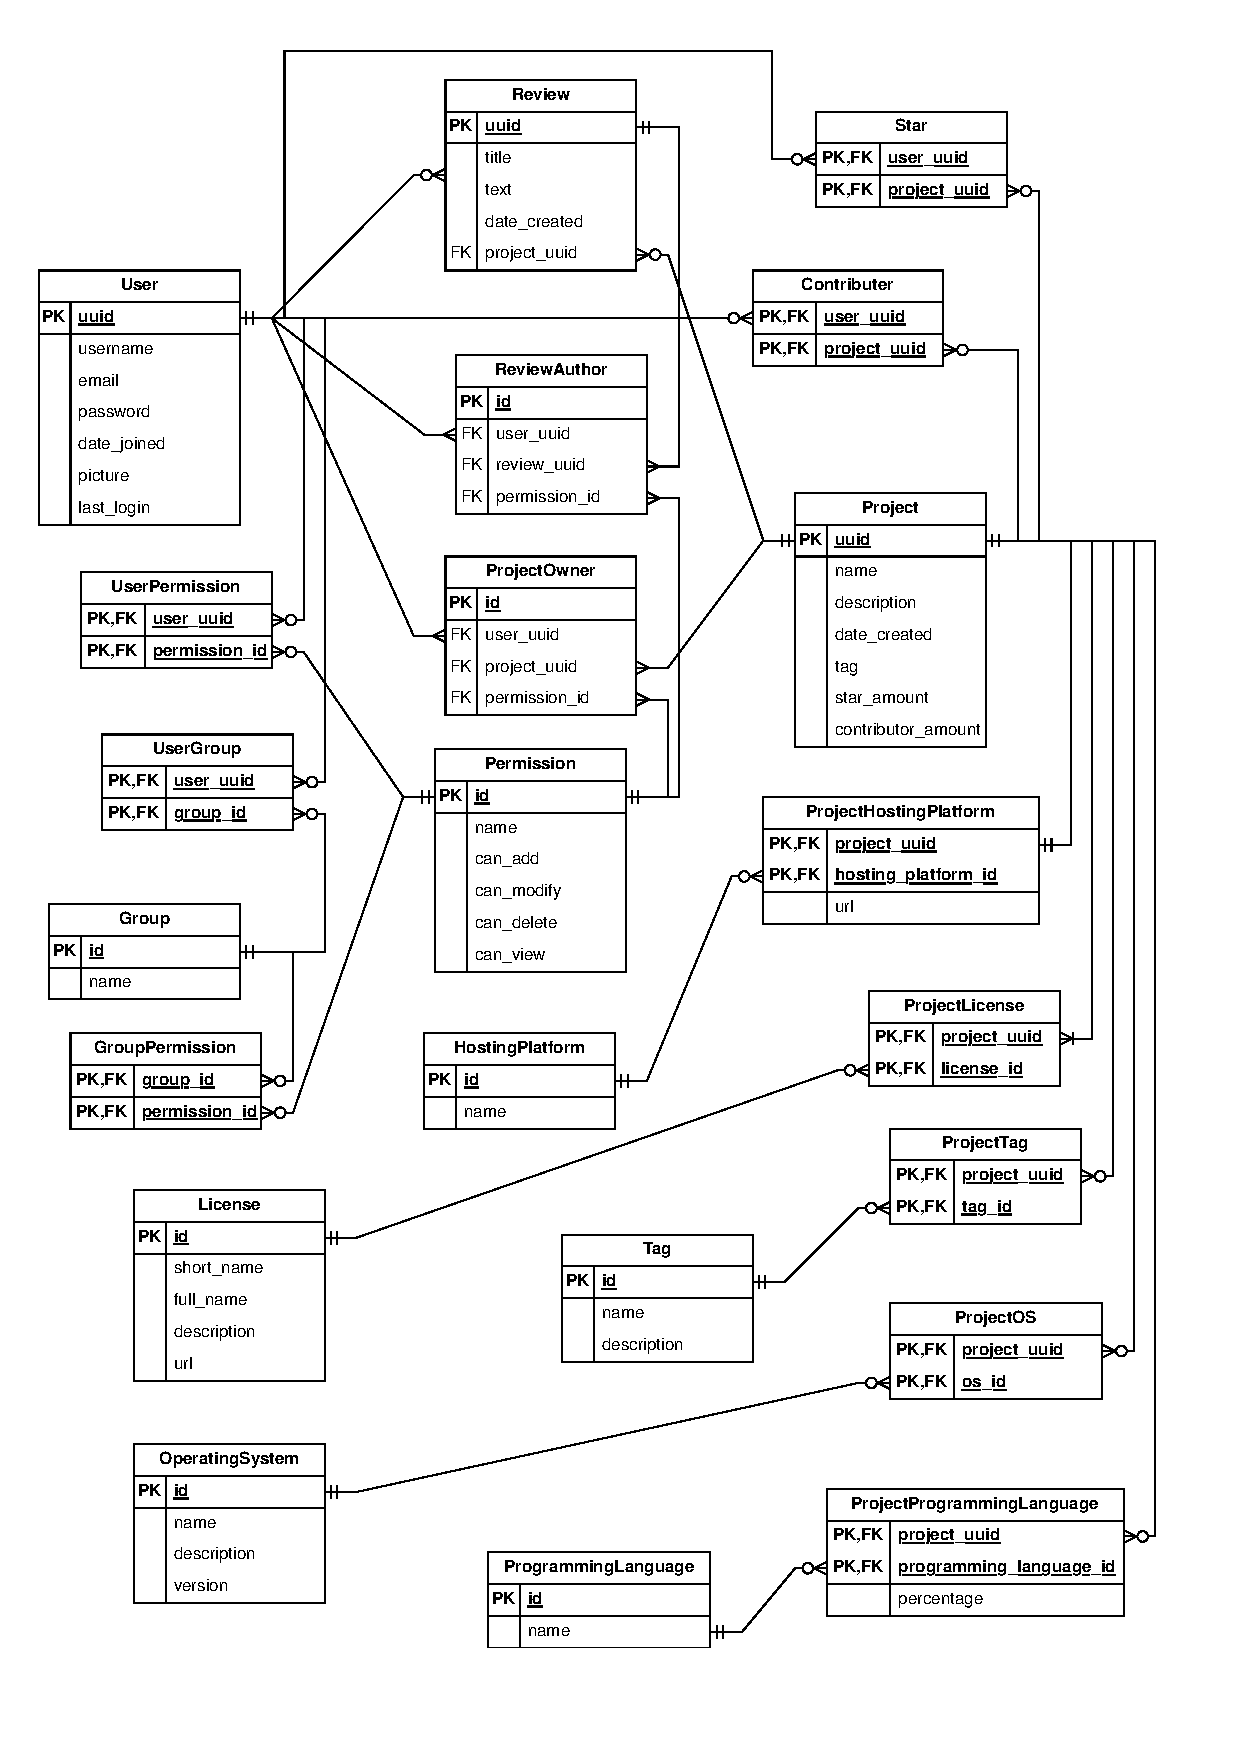
\includegraphics[width=0.8\textwidth]{./TeX-files/ERD/logical-model.pdf}
  \caption{Logical model}
  \label{fig:ERD}
\end{figure}

    % \input{./TeX-files/after-content/literature.tex}
\end{document}

